\chapter{Diagramme de classes}
\cfoot{}
\rfoot{}

La méthode GTD permet d'organiser les tâches selon plusieurs critères :\\

\begin{itemize}
\item le projet
\item le contexte (l’endroit, l’outil ou l’environnement dans lequel la tâche peut être réalisée)
\item la priorité
\item l'état d'avancement (à faire, déléguée, en attente, finie)
\end{itemize}

\begin{figure}[H]
\begin{center}
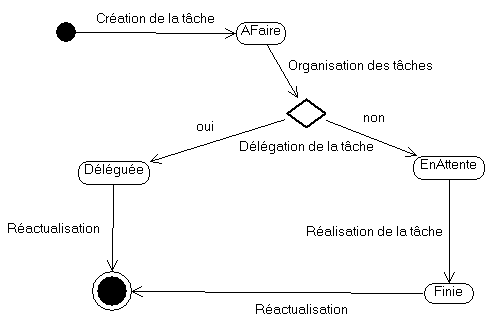
\includegraphics[scale=0.8]{diagrams/etats_tache.png}
\caption{Diagramme d'états transitions d'une tâche}
\end{center}
\end{figure}


Un projet regroupe donc des tâches et éventuellement, des sous-projets. A l’intérieur d’un projet, les tâches peuvent être indépendantes les unes des autres ou organisées en séquence. Un projet possède un nom, des notes, et peut préciser le contexte par défaut des nouvelles tâches du projet.
Une tâche possède différents attributs : \\
\begin{itemize}
\item son nom
\item une date de début
\item une échéance
\item des notes
\item une priorité (valeur comprise entre 1 et 5)
\item un taux d’effort demandé (valeur comprise entre 0 et 99)
\item une liste de contacts
\item une fréquence de répétition (journalière, hebdomadaire, mensuelle)
\item une date d’arrêt de la répétition
\item des liens (URLs) vers d’autres ressources
\item des tags
\item un et un seul contexte
\end{itemize} 


\begin{figure}[H]
\begin{center}
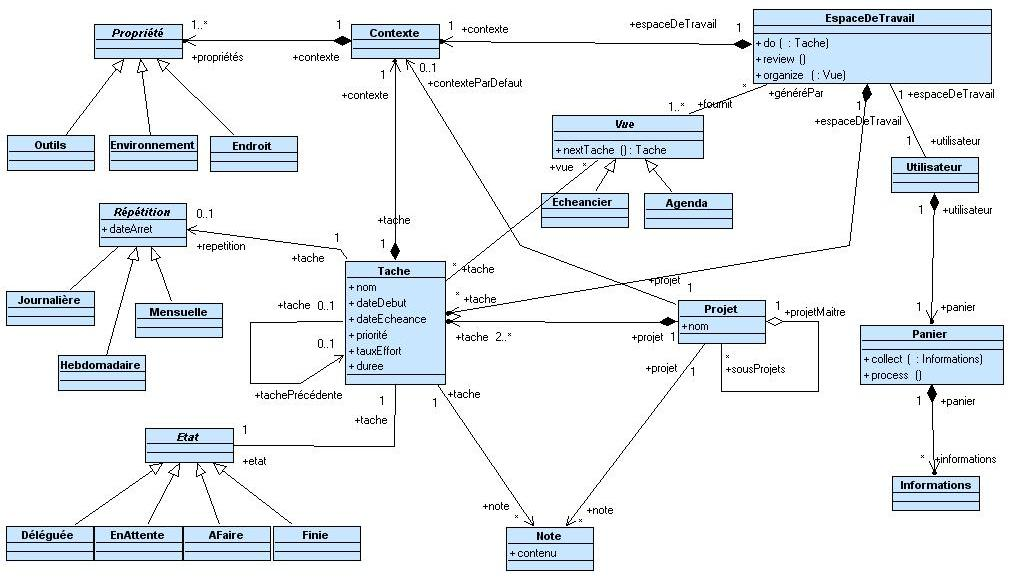
\includegraphics[scale=0.5,angle=90]{diagrams/diag_class.png}
\caption{Diagramme UML de classe}
\end{center}
\end{figure}



\cfoot{\thepage}
\rfoot{Celton,Hervouet,Levin,Vaillant}
\section{Contraintes OCL et explications}


	Les deux classes centrales sont \textbf{Projet} et \textbf{Tache}. Un projet peut inclure des sous-projets et ce récursivement. Un projet peut aussi contenir une séquence de tâches, dans ce cas les tâches sont vues sous formes d'une liste châinée. Seules les tâches d'un projet peuvent être séquencées :\\
\begin{lstlisting}
context Tache
	inv :
		self.projet->empty() implies self.tachePrécédente->empty() and
		self.tachePrécédente->notEmpty() implies self.tachePrécédente != self and
		self.projet->notEmpty() implies self.projet = self.tachePrécédente.projet and
		self.dateDebut <= self.dateEcheance and
		self.dateEchance >= self.repetition.dateArret and
		self.tauxEffort >= 0 and
		self.tauxEffort <= 99 and
		self.priorité >= 1 and
		self.priorité <= 5 and
		self.duree <= (self.dateEcheance - self.dateDebut)
\end{lstlisting}

	Un projet possède aussi un \textbf{contexteParDéfaut}, c'est à dire que tous ses sous-projets ainsi que toutes ses tâches incluent son contexte dans le leur :\\
\begin{lstlisting}
context Projet
	inv :
		self.contexteParDefaut.proprietes->notEmpty() implies
		(self.tache->forAll(each | each.contexte.proprietes->includesAll(self.contexteParDefaut.proprietes)) and
		self.sousProjet->forAll(each | each.contexte.proprietes->includesAll(self.contexteParDefaut.proprietes)))
\end{lstlisting}

	Pour effectuer la tâche courante, si celle-ci est séquencée, les tâches la précédant doivent être dans l'état \textbf{Finie}. Elle doit aussi être réalisable :\\
\begin{lstlisting}
context EspaceDeTravail::do(t : Tache)
	pre :
		t.tachePrécédente->notEmpty() implies t.tachePrécédente.oclInState(Finie) and
		t.tachePrécédente.oclInState(Finie) and
		not(t.oclInState(Finie)) and
		self.contexteCourant.propriétés->includesAll(t.contexte.propiétés)
	post :
		t.oclInState(Finie)
\end{lstlisting}

	La tâche courante est fournie à l'\textbf{Utilisateur} par la \textbf{Vue} de l'\textbf{EspaceDeTravail} en fonction de l'ordre chronologique (\textbf{Agenda}), des priorités (\textbf{Echeancier})...\\
\begin{lstlisting}
context Vue
	inv :
		self.generePar.tache->includesAll(self.tache)
		
context Vue::nextTache() : Tache
	post : 
		result = self.tache->first()
\end{lstlisting}

	C'est l'espace de travail qui offre la possibilité à l'utilisateur d'organiser les tâches en fonction des contextes, projets, dépendances (création de séquencement)...
\begin{lstlisting}
context EspaceDeTravail::organise(v : Vue)
	post :
		v.tache = v.tache@pre->asOrderedSet() and
		self.tache->forAll(each | (each@pre.oclInState(AFaire)) implies (each.oclInState(EnAttente)))
\end{lstlisting}

	Il offre aussi la possibilité de réactualiser l'ensemble des informations :
\begin{lstlisting}
context EspaceDeTravail::review()
	post :
		self.tache->notExists(each | each.oclInState(Finie))
\end{lstlisting}

	Le \textbf{Panier} représente le conteneur dans lequel l'utilisateur va noter (\textbf{collect(:Informations)}) tout événements, objets, documents ou idées (\textbf{Informations}) qui pourraient requérir une action ultérieure. Ces informations sont ensuite traitées par la méthode \textbf{process()}. Celle-ci crée les tâches correspondantes aux informations si c'est pertinent :
\begin{lstlisting}
context Panier::process()
	post :
		self.informations->empty()
\end{lstlisting}